\section{Results}

\begin{figure}[]
	\centering
	\begin{tabular}{cc}
		\subfloat{\includegraphics[width=0.5\textwidth]{images/BestOverlayGround}}&
		\subfloat{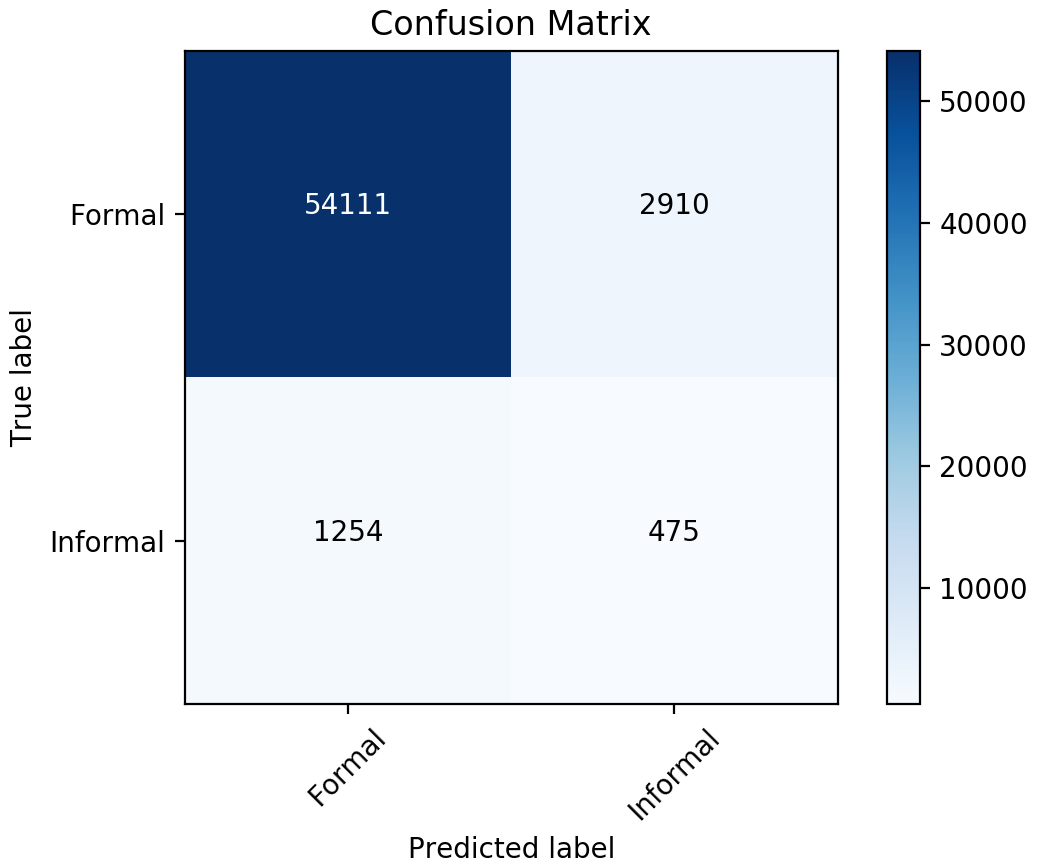
\includegraphics[width=0.57\textwidth]{images/BestConfusion}}
	\end{tabular}
	\caption{Classification of Section 2 using HoG and Gradient boosting}
	\label{fig:res_best}
\end{figure}

As we have described in the previous section, we perform multiple experiments to evaluate the performance of the feature classification under varying parameters. The maximum performance we were able to obtain is illustrated in Figure \ref{fig:res_best}; the red shapes are the areas that are confirmed as slum, the yellow parts are the areas that are predicted as slum. This resulted in an F1-Score of 0.19 and a Matthews coefficient of 0.17 using the second section as test image with the HoG features; the scales 50, 100 and 150; and Gradient boosting. The confusion matrix in the same figure displays the number of correct and incorrect classifications. In the next sections, we will discover the effects of various parameters on the classification performance.

\pgfplotstableread[col sep = comma]{results/features_sections.csv}\datazero

\begin{figure}[]
	\begin{tikzpicture}
	\begin{axis}[
	ybar,
	ymajorgrids = true,
	bar width=0.5cm,
	ylabel = Matthews Coefficient,
	width=\textwidth,
	height=.5\textwidth,
	enlarge x limits=0.25,
	symbolic x coords={Section 1, Section 2, Section 3},
	xtick=data,
	ymax = 1,
	yticklabel style={
		/pgf/number format/fixed,
		/pgf/number format/precision=2,
		/pgf/number format/fixed zerofill
	},
	scaled y ticks=false,
	]
	\addplot table[x=TestImage, y=HoG]{\datazero};
	\addplot table[x=TestImage, y=LSR]{\datazero};
	\addplot table[x=TestImage, y=RID]{\datazero};
	\addplot table[x=TestImage, y=All features]{\datazero};
	%\addplot[dotted, sharp plot, update limits=false] coordinates {(0, 0)(1, 0)}; 
	\legend{HoG, LSR, RID, All features}
	\end{axis}
	
	\end{tikzpicture}
	\caption{The performance of features measured by Matthews Coefficient}
	\label{fig:res_bar_0}
\end{figure}

\subsection{Feature Performance}

Because we use combinations of sections and features, the performance is likely to vary between different parameter combinations. We display the classification performance of all combinations of test images and features in Figure \ref{fig:res_bar_0} to discover the influence of the features and sections on performance. To reduce the complexity of the bar chart, we only display the results of the classifier with the highest performance and use the Matthews coefficient as the sole metric. In the experiment, HoG achieves the highest performance for all three sections. LSR seems to be more variable in performance than HoG over the three sections, although it is close to the performance of HoG in section 2. In contrast, RID achieves low performance for all sections. Lastly, the combination of all features performs slightly less than HoG in all three sections.


\pgfplotstableread[col sep = comma]{results/classifiers.csv}\dataone

\begin{figure}[]
	\begin{tikzpicture}
	\begin{axis}[
	ybar,
	bar width=.5cm,
	width=\textwidth,
	height=.5\textwidth,
	ymajorgrids = true,
	legend pos = north west,
	ylabel= Maximum Performance,
	symbolic x coords={DecisionTree, RandomForrest, AdaBoost, GradientBoost,MLP},
	xtick=data,
	yticklabel style={
		/pgf/number format/fixed,
		/pgf/number format/precision=2,
		/pgf/number format/fixed zerofill
	},
	scaled y ticks=false,
	]
	\addplot table[x=Classifier,y=F1-Score]{\dataone};
	\addplot table[x=Classifier,y=Matthews]{\dataone};
	
	
	\legend{F1-Score, Matthews Coefficient}
	\end{axis}
	
	\end{tikzpicture}
	\caption{Maximum Performance of the Classification Algorithms for all sections}
	\label{fig:res_bar_1}
\end{figure}

\subsection{Classifier Performance}

Although Figure \ref{fig:res_bar_0} shows the maximum performance of the features, it does not display the performance of the individual classifiers. We, therefore, compare the classification algorithms side by side to gain more insight into the performance differences between the classification algorithms that are displayed in Figure \ref{fig:res_bar_1}. The performance was measured used the maximum of the Matthews coefficient and the F1-score the classifier had achieved for any test image or feature. It turned out that, for all classifiers, the set of parameters that produced the maximum of Matthews Coefficient was the same set of parameters for the maximum F1-score, which seems to suggest that two measures of performance are consistent with each other.

Gradient boosting was able to produce achieve the highest performance, followed by MLP and AdaBoost. The Decision Tree and Random Forrest had the lowest maximum performance, although the order in performance is not necessarily definite, as is illustrated by the Figures \ref{fig:res_plot_0} and \ref{fig:res_bar_2}.

\begin{figure}[]
	\centering
	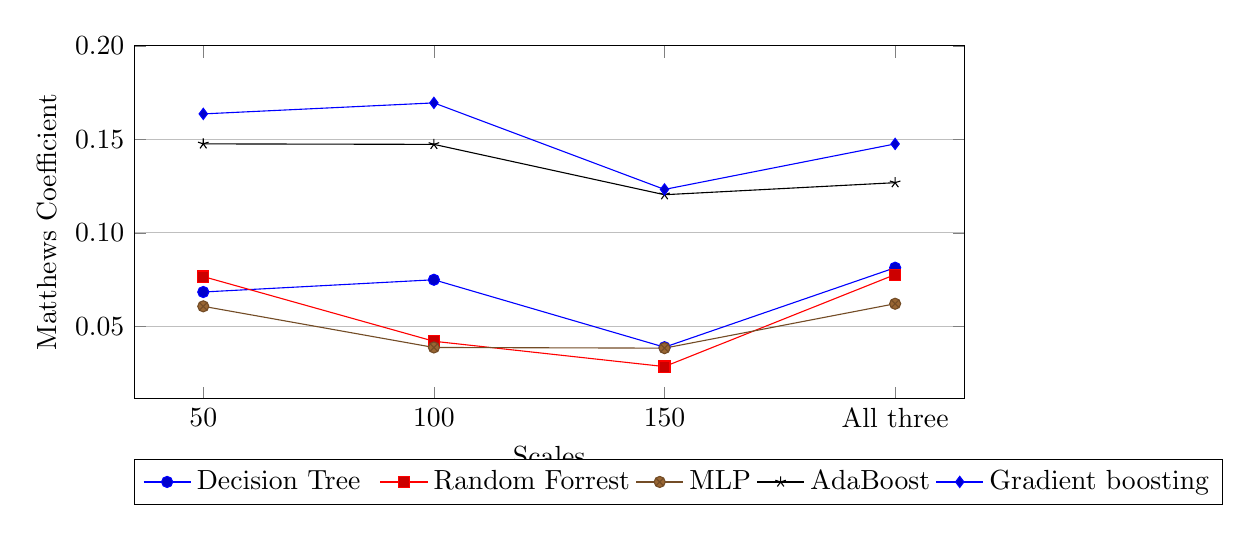
\begin{tikzpicture}
	\begin{axis}[
	title={},
	xlabel={Scales},
	ylabel={Matthews Coefficient},
	width=\textwidth,
	height=.5\textwidth,
	symbolic x coords={50, 100, 150, All three},
	xtick=data,
	ytick={-0.05, 0.0, 0.05, 0.10, 0.15, 0.20},
	yticklabel style={
		/pgf/number format/fixed,
		/pgf/number format/precision=2,
		/pgf/number format/fixed zerofill
	},
	ymax=0.20,
	legend pos=north west,
	ymajorgrids=true,
	legend columns=5, 
	legend style={
		% the /tikz/ prefix is necessary here...
		% otherwise, it might end-up with `/pgfplots/column 2`
		% which is not what we want. compare pgfmanual.pdf
		/tikz/column 2/.style={
			column sep=5pt,
		},
		at={(0.0, -0.17)},
	}
	]
	
	\addplot
	coordinates {
		(50,0.068427407212623)(100, 0.074966895103175)(150, 0.038928267316005)(All three, 0.081409428624833)
	};
	
	\addplot
	coordinates {
		(50, 0.076677199288863)(100, 0.042099627073353)(150, 0.028570812585408)(All three, 0.077733110578942)
	};
	
	\addplot
	coordinates {
		(50,0.060778260530553)(100, 0.038786124761983)(150, 0.038425470626755)(All three, 0.062153606915537)
	};
	\addplot
	coordinates {
		(50, 0.147590307870466)(100,0.147328964006612)(150, 0.120414247378828)(All three, 0.126851482904826)
	};
	\addplot
	coordinates {
		(50, 0.163610733799053 )(100, 0.169491852975136)(150, 0.123248189675469)(All three, 
		0.147566516221729)
	};
	\legend{Decision Tree, Random Forrest, MLP, AdaBoost, Gradient boosting}
	
	
	\end{axis}
	\end{tikzpicture}
	\caption{Effects of scale on classification performance}
	\label{fig:res_plot_0}
\end{figure}

\subsection{Effect of different Scales}

As we have discussed in the feature evaluation, we suspect increased scale to have a positive effect on the classification performance of the features. In this experiment, the only variable is a different scale. The other constant parameters are section 2 as the test image, a block size of 20 and all features. We chose this set of parameters because it has shown to produced adequate results in the previous experiment, as displayed in Figure \ref{fig:res_bar_0}. The results of the experiment in Figure \ref{fig:res_plot_0} seems to indicate that increased scale does not necessarily result in improved performance. However, we performed the same experiment using Section 1 as test image and did see a slight improvement of performance.


\pgfplotstableread[col sep = comma]{results/block_size.csv}\datatwo

\begin{figure}[]
	\begin{tikzpicture}
	\begin{axis}[
	%ybar,
	%bar width=.5cm,
	width=\textwidth,
	height=.5\textwidth,
	ymajorgrids = true,
	legend pos = north west,
	ylabel={Matthews Coefficient},
	symbolic x coords={10, 20, 40, 60},
	xtick=data,
	xlabel={Block Size},
	yticklabel style={
		/pgf/number format/fixed,
		/pgf/number format/precision=2,
		/pgf/number format/fixed zerofill
	},
	scaled y ticks=false,
	legend columns=5, 
	legend style={
		/tikz/column 2/.style={
			column sep=5pt,
		},
		at={(0.0, -0.17)},
	}
	]
	\addplot table[x=Block Size, y=DecisionTreeClassifier]{\datatwo};
	\addplot table[x=Block Size, y=RandomForestClassifier]{\datatwo};
	\addplot table[x=Block Size, y=MLPClassifier]{\datatwo};
	\addplot table[x=Block Size, y=AdaBoostClassifier]{\datatwo};
	\addplot table[x=Block Size, y=GradientBoostingClassifier]{\datatwo};
	
	\legend{DecisionTree, RandomForest, MLP, AdaBoost, Gradient boosting}
	\end{axis}
	
	\end{tikzpicture}
	\caption{The effects of the block size on classification performance}
	\label{fig:res_bar_2}
\end{figure}

\subsection{Effect of different Block sizes}
In the feature evaluation section, we observed that increased block size did not seem to influence the difference between the formal and informal value distributions. Being able to use a large block size while maintaining similar results is highly preferable to a small block size as the computational cost increases squared for a linear decrease in block size. We will evaluate if our observation from the feature evaluation translates to constant performance with a decreasing computational load. Besides the block sizes used in the feature evaluation section, we also run the experiment with a block size of 10 to discover if this might improve performance. The experiment uses the constant parameters: section 2 as the test image, all three features, and the scales 50, 100 and 150. The variable parameter in this experiment is the block size, which is tested on performance for the values 10, 20, 40 and 60. The results of the experiment are displayed in Figure \ref{fig:res_bar_2} and, as we have hypothesized, an increase in the block size generally does not seem to reduce performance. A reduction in block size to 10 seems to significantly reduce performance for all classifiers, except for the decision tree, which has relatively constant performance for all tested block sizes.



\pgfplotstableread[col sep = comma]{results/oversampling.csv}\datathree

\begin{figure}[]
	\begin{tikzpicture}
	\begin{axis}[
	ybar,
	bar width=.5cm,
	width=\textwidth,
	height=.5\textwidth,
	ymajorgrids = true,
	legend pos = north west,
	ylabel= Maximum Performance,
	symbolic x coords={Nothing, Random, ADASYN, SMOTE},
	xtick=data,
	yticklabel style={
		/pgf/number format/fixed,
		/pgf/number format/precision=2,
		/pgf/number format/fixed zerofill
	},
	scaled y ticks=false,
	]
	\addplot table[x=Methods,y=F1-Score]{\datathree};
	\addplot table[x=Methods,y=Matthews]{\datathree};
	
	\legend{F1-Score, Matthews Coefficient}
	\end{axis}
	
	\end{tikzpicture}
	\caption{The effect of oversampling on classification performance}
	\label{fig:res_bar_3}
\end{figure}

\subsection{Effects of oversampling}
In this experiment, we compare the three different oversampling methods to the performance achieved without oversampling, which are: random oversampling, SMOTEBoost and ADASYN. We performed the experiment with the default parameters displayed in Figure \ref{fig:params} with the second section as test image and a variable oversampling method. The performance of these parameters is displayed in Figure \ref{fig:res_bar_3}, which seems to indicate that any oversampling method increases the classification performance to the same extent, regardless of the method used.




